\section{System Design and Implementation}
\subsection{NFV Design Overview}
With the concept of SDN-enabled VNFs in Fig. \ref{fig:vnf_overview}, the network functions have been achived by the synergies between compute and network infrastructures. The former is mainly responsible for dealing with stateful processing, and the latter is used for stateless processing component.

\subsubsection{Stateful Processing Componemt}
This component have to perform more complex algorithm, keep the state associated with the VNF and provide interface for service providers or customers to configure and update the behavior of the stateless datapath processing component, since software is good at these tasks. It's worth noting that we use southbound APIs of SDN controller to handle the interface between the stateful and stateless component with OpenFlow protocol, which was originally designed for this.

\subsubsection{Stateless Processing Componemt}
Stateless processing component, are implemented by SDN datapath resources, which is optimized for data plane traffic processing. Since SDN datapath have decoupled the control plane and data plane, so it can accept the control message from the stateful processing component.

\begin{figure}[!t]
  \centering
  \def\svgwidth{\linewidth}
  \input{figures/nfv_overview.pdf_tex}
  \caption{NFV design overview}
  \label{fig:vnf_overview}
\end{figure}

\subsection{Architecture of the vCPE Platform}

\subsubsection{System Overview}
See Fig \ref{fig:vcpe_overview}
\begin{figure}[!t]
  \centering
  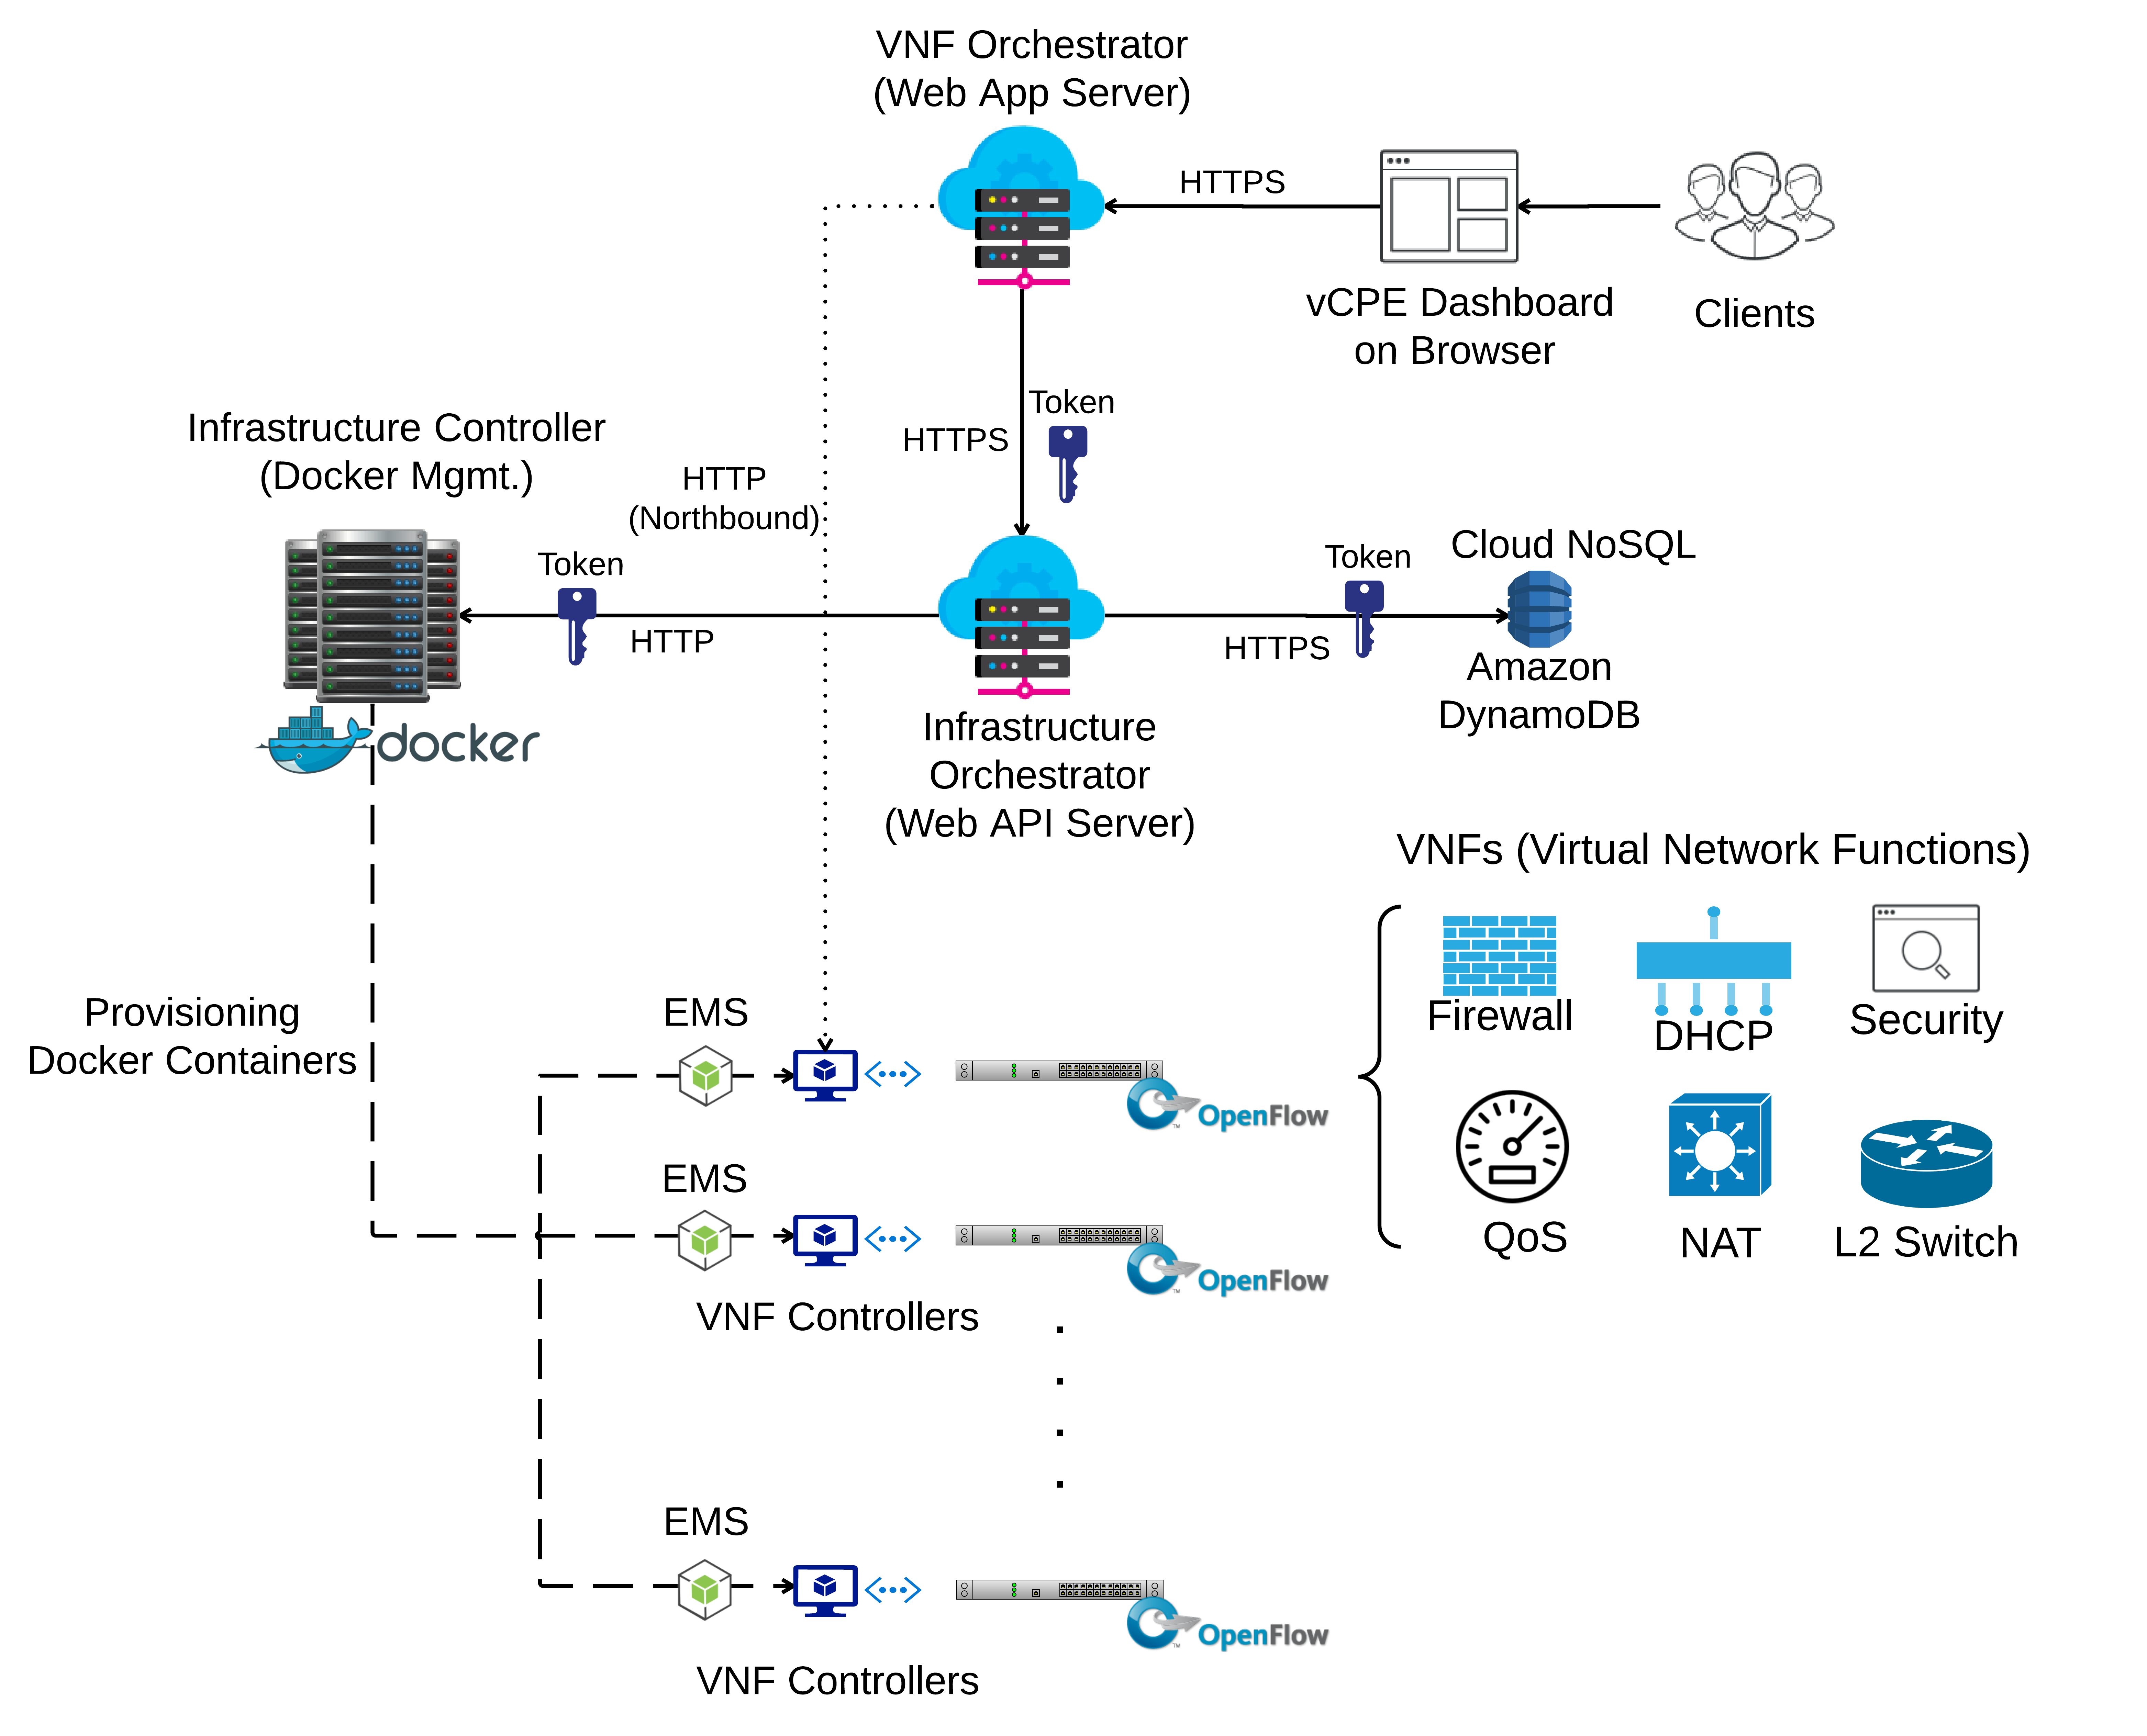
\includegraphics[width=\linewidth]{./figures/system-overview}
  \caption{vCPE platform overview}
  \label{fig:vcpe_overview}
\end{figure}

\subsubsection{System Implementation}
\begin{enumerate}[1)]
  \item{\bf{Infrastructure Orchiestrator}}
  \item{\bf{Infrastructure Controller}}
  \item{\bf{VNF Orchiestrator}}
  \item{\bf{VNF Controllers}}
\end{enumerate}
